
Gazebo, an open-source \acs{3d} robotics simulator, makes it possible for developers to rapidly test algorithms, design robots, 
perform regression testing, 
and train \acs{ai} systems using realistic scenarios. In gazebo the developer can create custom environments. 
These environments have realistic rendering including high-quality lighting, shadows, and textures. 
Sensors that can see the simulated environment on robots can be modeled \cite{gazebo:org}.

\begin{figure}[ht]
    \centering
    
\includegraphics[scale = 0.6]{gazebo.png}
    \caption[Gazebo logo]{Gazebo logo\footnotemark.}
\end{figure}

\begin{figure}[ht]
    \centering
    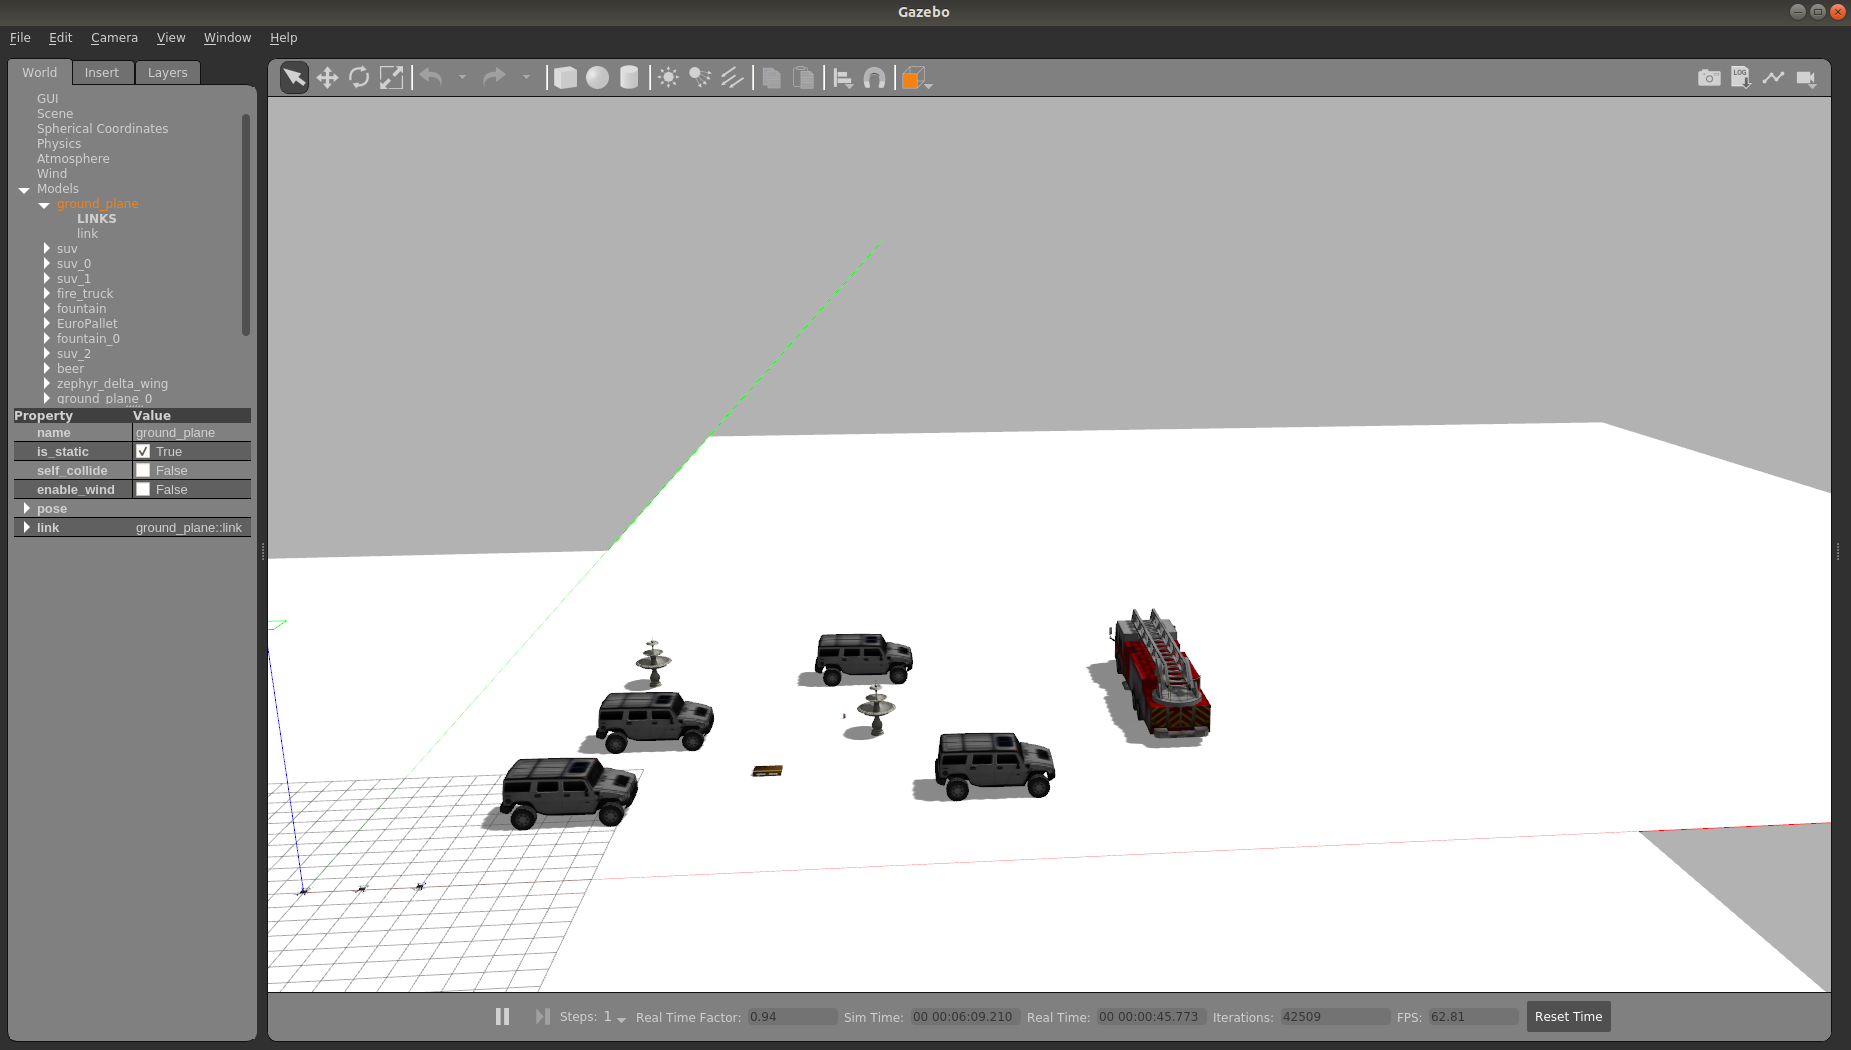
\includegraphics[scale = 0.2]{gazebo_full_screen.png}
    \caption[Gazebo Simiulation with 3 UAVs]{Gazebo Simiulation\footnotemark.}
\end{figure}
\newpage